

    \item Two identical glass rods \( S_1 \) and \( S_2 \) (refractive index = 1.5) have one convex end of radius of curvature 10 cm. They are placed with the curved surfaces at a distance \( d \) as shown in the figure, with their axes (shown by the dashed line) aligned. When a point source of light \( P \) is placed inside rod \( S_1 \) on its axis at a distance of 50 cm from the curved face, the light rays emanating from it are found to be parallel to the axis inside \( S_2 \). The distance \( d \) is
    \begin{center}
        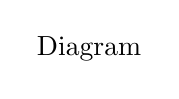
\begin{tikzpicture}
            \node {Diagram};
        \end{tikzpicture}
    \end{center}
        \begin{tasks}(2)
            \task 60 cm
            \task 70 cm
            \task 80 cm
            \task 90 cm
        \end{tasks}
        

